\newcommand{\rts}{\ \dashv\ }

% eugene:
%
% like
% not your typical
% tofte talpin how to pronounce
% {r} explain
% merge 7, 8 or make {r} a comment
% regions: coloring for new stuff
% better explanatino of qualifiers (examples?)
% better arrows for isolated+immutable picture
% too much update/collection-cycle explanations
% snapshot
%   heap state -> heap address
%   time       -> observed time
% too much text research proposal part
% opaque pronounciation
% extra slides to replace questions
%
% dima:
%
% explain region open vs evidence
% explain when region evidence is not needed
% consider reordering reference qualifiers: swap immutable and writable
% explain isolated-immutable reference
% 4 nulls
% explain RemIso
% remiso
% no synchronization in write barrier, not no synchronization at all
% new slide! explain when to deallocate separate slide
% explain _i == thread number i
% ownership vs regions about the same?
% comparison table message not clear
% too much discussion summary

\title{Safe Low-Overhead Memory Management for Concurrency and Parallelism}
\author{Denys Shabalin}
\date{21 July 2015}
{
\setbeamertemplate{footline}{}
\begin{frame}
    \titlepage
\end{frame}
}


\begin{frame}
    \frametitle{Overview}
    \begin{enumerate}
        \item Region-based memory in Cyclone
        \item Uniqueness and reference immutability for safe parallelism
        \item An efficient on-the-fly cycle collection
        \item Research proposal
    \end{enumerate}
\end{frame}

\begin{frame}
    \begin{center}
        {\LARGE Region-based memory in Cyclone} \\
        \vspace{20pt}
        Dan Grossman, Michael Hicks, Greg Morrisett,\\
        Yanling Wang, Trevor Jim, James Cheney
    \end{center}
\end{frame}

\begin{frame}
    \frametitle{Safe region-based memory management}

    Pioneered by M. Tofte and J.P. Talpin who explored the concept in functional
    programming languages of the ML family.
\end{frame}

\begin{frame}
    \frametitle{Cyclone overview}
    \begin{itemize}
        \item Close to C syntactically to ease porting of existing programs.
        \item Adds tagged unions, polymorphism, \textit{regions} etc.
        \item Guarantees memory safety via static type checking.
    \end{itemize}
\end{frame}

\begin{frame}[fragile]
    \frametitle{Regions in Cyclone}
    \begin{verbatim}
    void main() {
        region r {
            struct Point*r p = rnew(r) { 10.0, 10.0 };
            printf("Point at (%d, %d)", p->x, p->y);
        }
    }
    \end{verbatim}
\end{frame}

\begin{frame}[fragile]
    \frametitle{Regions in Cyclone}
    \begin{verbatim}
    void main() {
        region r {
            struct Point*r p = rnew(r) { 10.0, 10.0 };
            printPoint<r>(p)
        }
    }

    void printPoint<r>(Point*r p) {
        printf("Point at (%d, %d)", p->x, p->y);
    }
    \end{verbatim}
\end{frame}

\begin{frame}[fragile]
    \frametitle{Regions in Cyclone}
    \begin{verbatim}
    void main() {
        region r {
            struct Point*r p = rnew(r) { 10.0, 10.0 };
            printPoint<r>(p)
        }
    }

    void printPoint<r>(Point*r p; {r}) {
        printf("Point at (%d, %d)", p->x, p->y);
    }
    \end{verbatim}
\end{frame}

\begin{frame}[fragile]
    \frametitle{Cyclone type system: abstract syntax}

    $\tau ::= \tau_1 \xrightarrow{\epsilon} \tau_2\ |
            \ \tau * \rho\ |\ handle(\rho)\ |\ ... $
    \\ \vspace{10pt}

    $e ::= x_\rho\ |\ *e\ |\ e_1(e_2)\ |\ rnew(e_1)\ e_2\ |\ ...$
    \\ \vspace{10pt}

    $s ::=  e\ |\ return\ e\ |\ s_1; s_2 |
            \ region \langle \rho \rangle\ x_\rho\ s\ |\ ...$
    \\ \vspace{10pt}

    $\Gamma ::= \bullet\ |\ \Gamma, x_\rho: \tau$
    \\ \vspace{10pt}

    $\Delta ::= \bullet\ |\ \Delta, \alpha: \kappa$
    \\ \vspace{10pt}

    $\gamma ::= \emptyset\ |\ \gamma, \epsilon <: \rho$
    \\ \vspace{10pt}

    $\epsilon ::= \alpha_1\ \cup\ \alpha_2\ \cup \ ...\ \cup\ \alpha_n \ \cup \
                  \{ \rho_1,\ ..., \rho_m \}$
    \\ \vspace{10pt}

    $C ::= \Gamma; \Delta; \gamma; \epsilon$
\end{frame}

\begin{frame}
    \frametitle{Cyclone type system: judgments}
    \begin{center}
    \begin{tabular}{c | c}
    Expression typing & $\Delta; \Gamma; \gamma; \epsilon \ts e: \tau$         \\
                      \hline
    Statement typing  & $\Delta; \Gamma; \gamma; \epsilon; \tau \ts_{stmt}\ s$ \\
                      \hline
    Region liveness   & $\gamma \ts \epsilon \Rightarrow \rho$                 \\
                      & $\gamma \ts \epsilon_1 \Rightarrow \epsilon_2$
    \end{tabular}
    \end{center}
\end{frame}

\begin{frame}
    \frametitle{Cyclone type system: typing pointer dereference}
    \infrule
    {
        \Delta; \Gamma; \gamma; \epsilon \ts e: \tau * \rho \ \ \ \
        \gamma \ts \epsilon \Rightarrow \rho
    }
    {
        \Delta; \Gamma; \gamma; \epsilon \ts *e: \tau
    }
\end{frame}

\begin{frame}
    \frametitle{Cyclone type system: typing function application}
    \infrule
    {
        \Delta; \Gamma; \gamma; \epsilon \ts
        e_1: \tau_2 \xrightarrow{\epsilon_1} \tau \ \
        \Delta; \Gamma; \gamma; \epsilon \ts
        e_2: \tau_2 \ \
        \gamma \ts \epsilon \Rightarrow \epsilon_1
    }
    {
        \Delta; \Gamma; \gamma; \epsilon \ts
        e_1 (e_2): \tau
    }
\end{frame}

\begin{frame}
    \frametitle{Cyclone: summary}

    \begin{itemize}
        \item
            Region based memory management ties memory management
            to explicitly delimited blocks of code
        \item
            Static safety is ensured through region-annotated reference
            types and simple effect checking
    \end{itemize}
\end{frame}

\begin{frame}
    \begin{center}
        {\LARGE Uniqueness and reference immutability\\ for safe parallelism} \\
        \vspace{20pt}
        Colin S. Gordon, Matthew J. Parkinson, \\
        Jared Parsons, Aleks Bromfield, Joe Duffy
    \end{center}
\end{frame}

\begin{frame}
    \frametitle{Uniqueness and reference immutability}
    Introduces reference qualifiers to the C\# language:
    \begin{itemize}
        \item \textbf{writable} T
        \item \textbf{readable} T
        \item \textbf{immutable} T
        \item \textbf{isolated} T
    \end{itemize}
\end{frame}

\begin{frame}
    \frametitle{Uniqueness and reference immutability}
    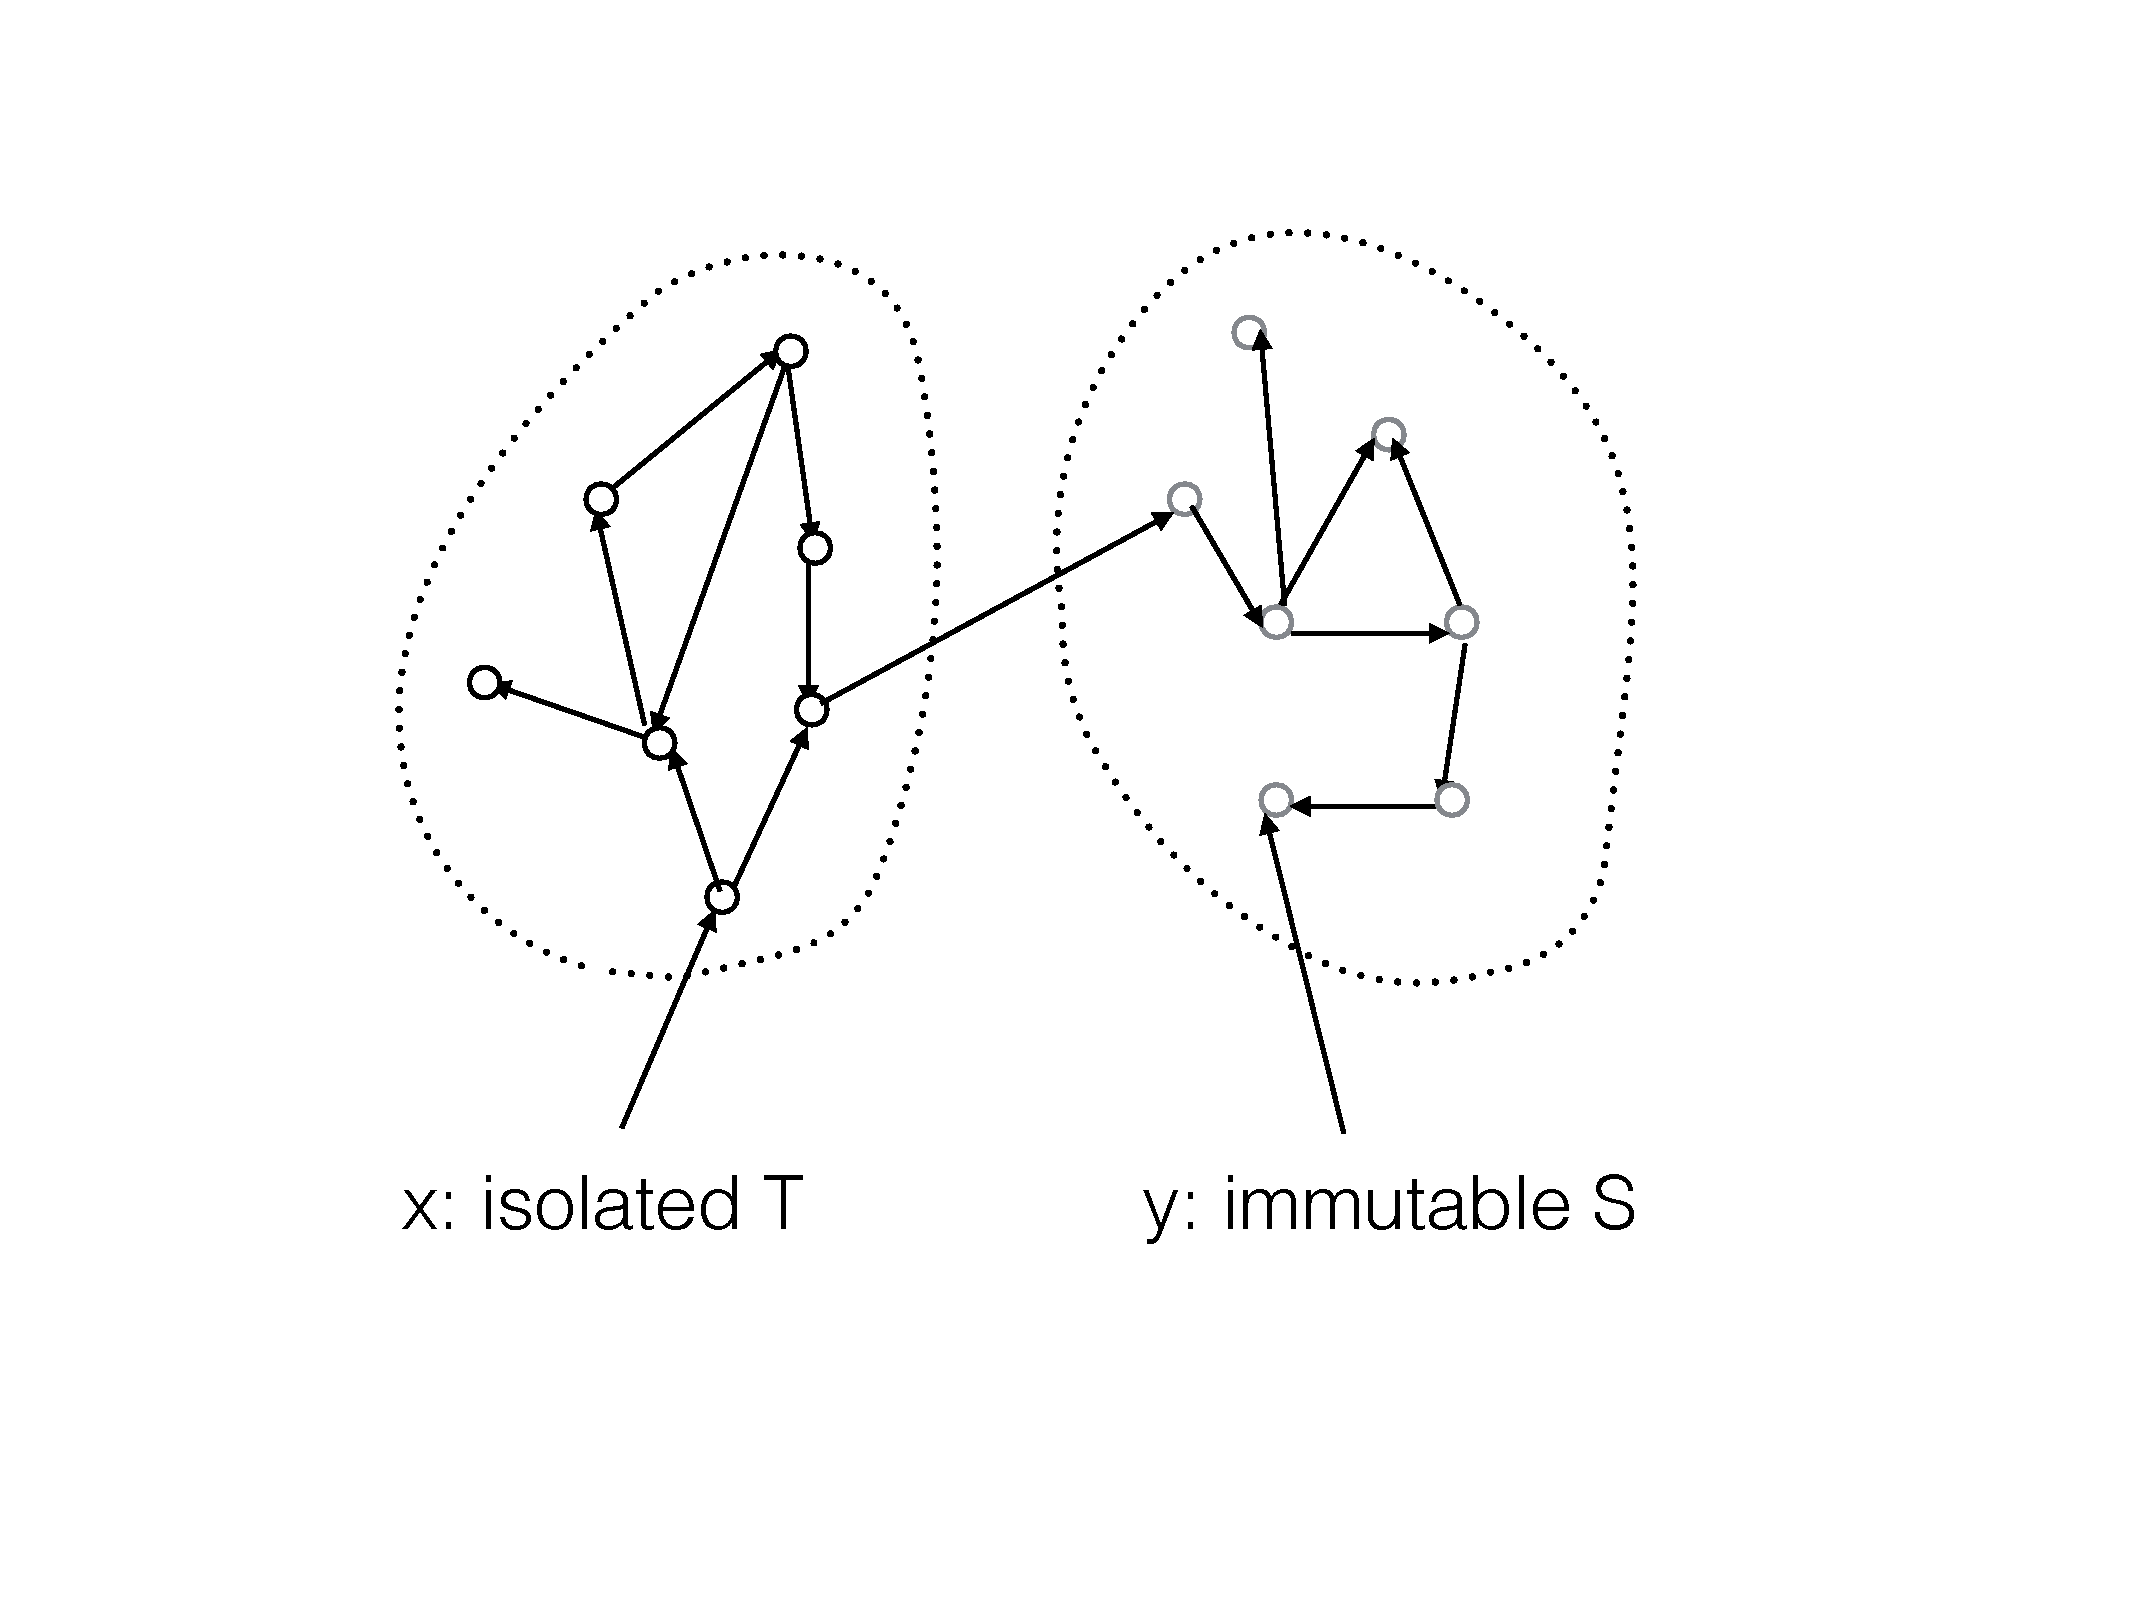
\includegraphics[width=350pt]{iso_imm.pdf}
\end{frame}

\begin{frame}
    \frametitle{Uniqueness and reference immutability: abstract syntax}

    $a ::= x = y\ |\ x.f = y\ |\ x = y.f\ |\ x = consume(y.f)\ |\ ...$

    $C ::= a\ |\ C; C\ |\ ...$

    $T ::= cn$

    $TD ::= class\ cn [<: T] \{\ fld*\ meth*\ \}$

    $p ::= readable\ |\ writable\ |\ immutable\ |\ isolated$

    $t ::= int\ |\ bool\ |\ p\ T$

    $\Gamma ::= \epsilon\ |\ \Gamma, x: t$
\end{frame}

\begin{frame}
    \frametitle{Uniqueness and reference immutability: judgements}
    \begin{center}
    \begin{tabular}{c | c}
    Command typing & $\Gamma \ts C \rts \Gamma$ \\
                   \hline

    Program typing & $\ts P$          \\
                   & $P \ts TD$       \\
                   & $P; TD \ts fld$  \\
                   & $P; TD \ts meth$ \\
                   \hline

    Subtyping & $\ts p \prec p'$    \\
              & $\ts T \prec T'$    \\
              & $\ts t_1 \prec t_2$ \\
              \hline

    Permission combination & $p_1 \rhd p_2 = p_3$                \\
                           & $p_1 \rhd p_2 T = (p_1 \rhd p_2) T$ \\
    \end{tabular}
    \end{center}
\end{frame}

\begin{frame}
    \frametitle{Uniqueness and reference immutability: typing}
    \infrule
    {
        t \neq isolated\ \_
    }
    {
        x: \_,\ y: t \ts x = y \rts y: t,\ x: t
    }
    \infrule
    {
        t'\ f \in T \\
        p \neq isolated \vee t' = immutable\ \_ \\
        t' \neq isolated\ \_ \vee p = immutable
    }
    {
        x: \_,\ y: p\ T
        \ts x = y.f
        \rts y: p\ T,\ x: p \triangleright t'
    }
    \infrule
    {
        t\ f \in T
    }
    {
        y: writable\ T,\ x: t
        \ts y.f = x
        \rts y: writable\ T,\ RemIso(x: t)
    }
    \infrule
    {
        isolated\ T_f \ f \in T
    }
    {
        y: writable\ T
        \ts x = consume(y.f)
        \rts y: writable\ T,\ x: isolated\ T
    }
\end{frame}

\begin{frame}
    \frametitle{Uniqueness and reference immutability: typing}
    \infrule
    {
        t'\ m(\seq{u'\ z'})\ p' \in T \ \ \ \
        \ts p \prec p' \ \ \ \
        \seq{\ts u \prec u'} \\
        p = isolated \Rightarrow \\
                 t \neq readable\ \_\
        \wedge\  t \neq writable\ \_\\
        \wedge\  IsoOrImm(\seq{z: t})\
        \wedge\  p' \neq immutable
    }
    {
        y: p\ T,\ \seq{z: u}
        \ts x = y.m(\seq{z})
        \rts y: p\ T,\ RemIso(\seq{z: t}),\ x: t'
    }
\end{frame}

\begin{frame}
    \frametitle{Uniqueness and reference immutability: applications}

    \begin{itemize}
        \item Statically enforced data-race freedom
        \item Optimizations of the GC due to known invariants
        \item Ownership-based memory management
    \end{itemize}
\end{frame}

\begin{frame}
    \begin{center}
        {\LARGE An efficient on-the-fly cycle collection} \\
        \vspace{20pt}
        Harel Paz, David F. Bacon, Elliot K. Kolodner,\\
        Erez Petrank, V. T. Rajan
    \end{center}
\end{frame}

\begin{frame}
    \frametitle{Efficient on-the-fly collection: previous work}
    \begin{enumerate}
        \item
            Yossi Levanoni and Erez Petrank.
            \textit{An on-the-fly reference counting garbage collection for Java}.
        \item
            David F. Bacon and V. T. Rajan.
            \textit{Concurrent cycle collection in reference counted systems}.
        \item
            Harel Paz, Erez Petrank, and Stephen M. Blackburn.
            \textit{Age-oriented concurrent garbage collection}.
    \end{enumerate}
\end{frame}

\begin{frame}
    \frametitle{1. On-the-fly ref. counting garbage collection for Java}

    Introduces two algorithms:
    \begin{enumerate}
        \item Stop-the-world snapshot algorithm
        \item On-the-fly sliding views algorithm
    \end{enumerate}
\end{frame}

\begin{frame}
    \frametitle{Stop-the-world snapshot collector}
    \begin{itemize}
        \item
            Reference counts are only heap-to-heap.
        \item
            No need to maintain reference counts between cycle collections.
            Out of multiple assignments \texttt{obj.slot = $v_1$, ..., $v_n$}
            \\ only \texttt{RC($v_1$) -= 1} and \texttt{RC($v_n$) += 1}
            are relevant.
        \item
            Instead of constantly maintaining reference counts lets
            just record old value for all of the fields that changed.
        \item
            To reclaim an object it must both have 0 reference count and
            not be referenced from stack or registers.
    \end{itemize}
\end{frame}

\begin{frame}[fragile]
    \frametitle{Stop-the-world snapshot algorithm}
    Synchronization-free write barrier:
    \begin{verbatim}

        Procedure Update(s: Slot, new: Object)
        begin
            local old := read(s)
            if not Dirty(s) then
                Buffer_i[CurrPos_i] := <s, old>
                CurrPos_i := CurrPos_i + 1
                Dirty(s) := true
            write(s, new)
        end
    \end{verbatim}
\end{frame}

\begin{frame}[fragile]
    \frametitle{Stop-the-world snapshot algorithm}
    Collector logic:
    \begin{verbatim}

        Procedure Collection-Cycle
        begin
            // Stop-The-World
            Read-Current-State
            Update-Reference-Counters
            Read-Buffers
            Fix-Undetermined-Slots
            Reclaim-Garbage
        end
    \end{verbatim}
\end{frame}

\begin{frame}
    \frametitle{On-the-fly sliding views collector}
    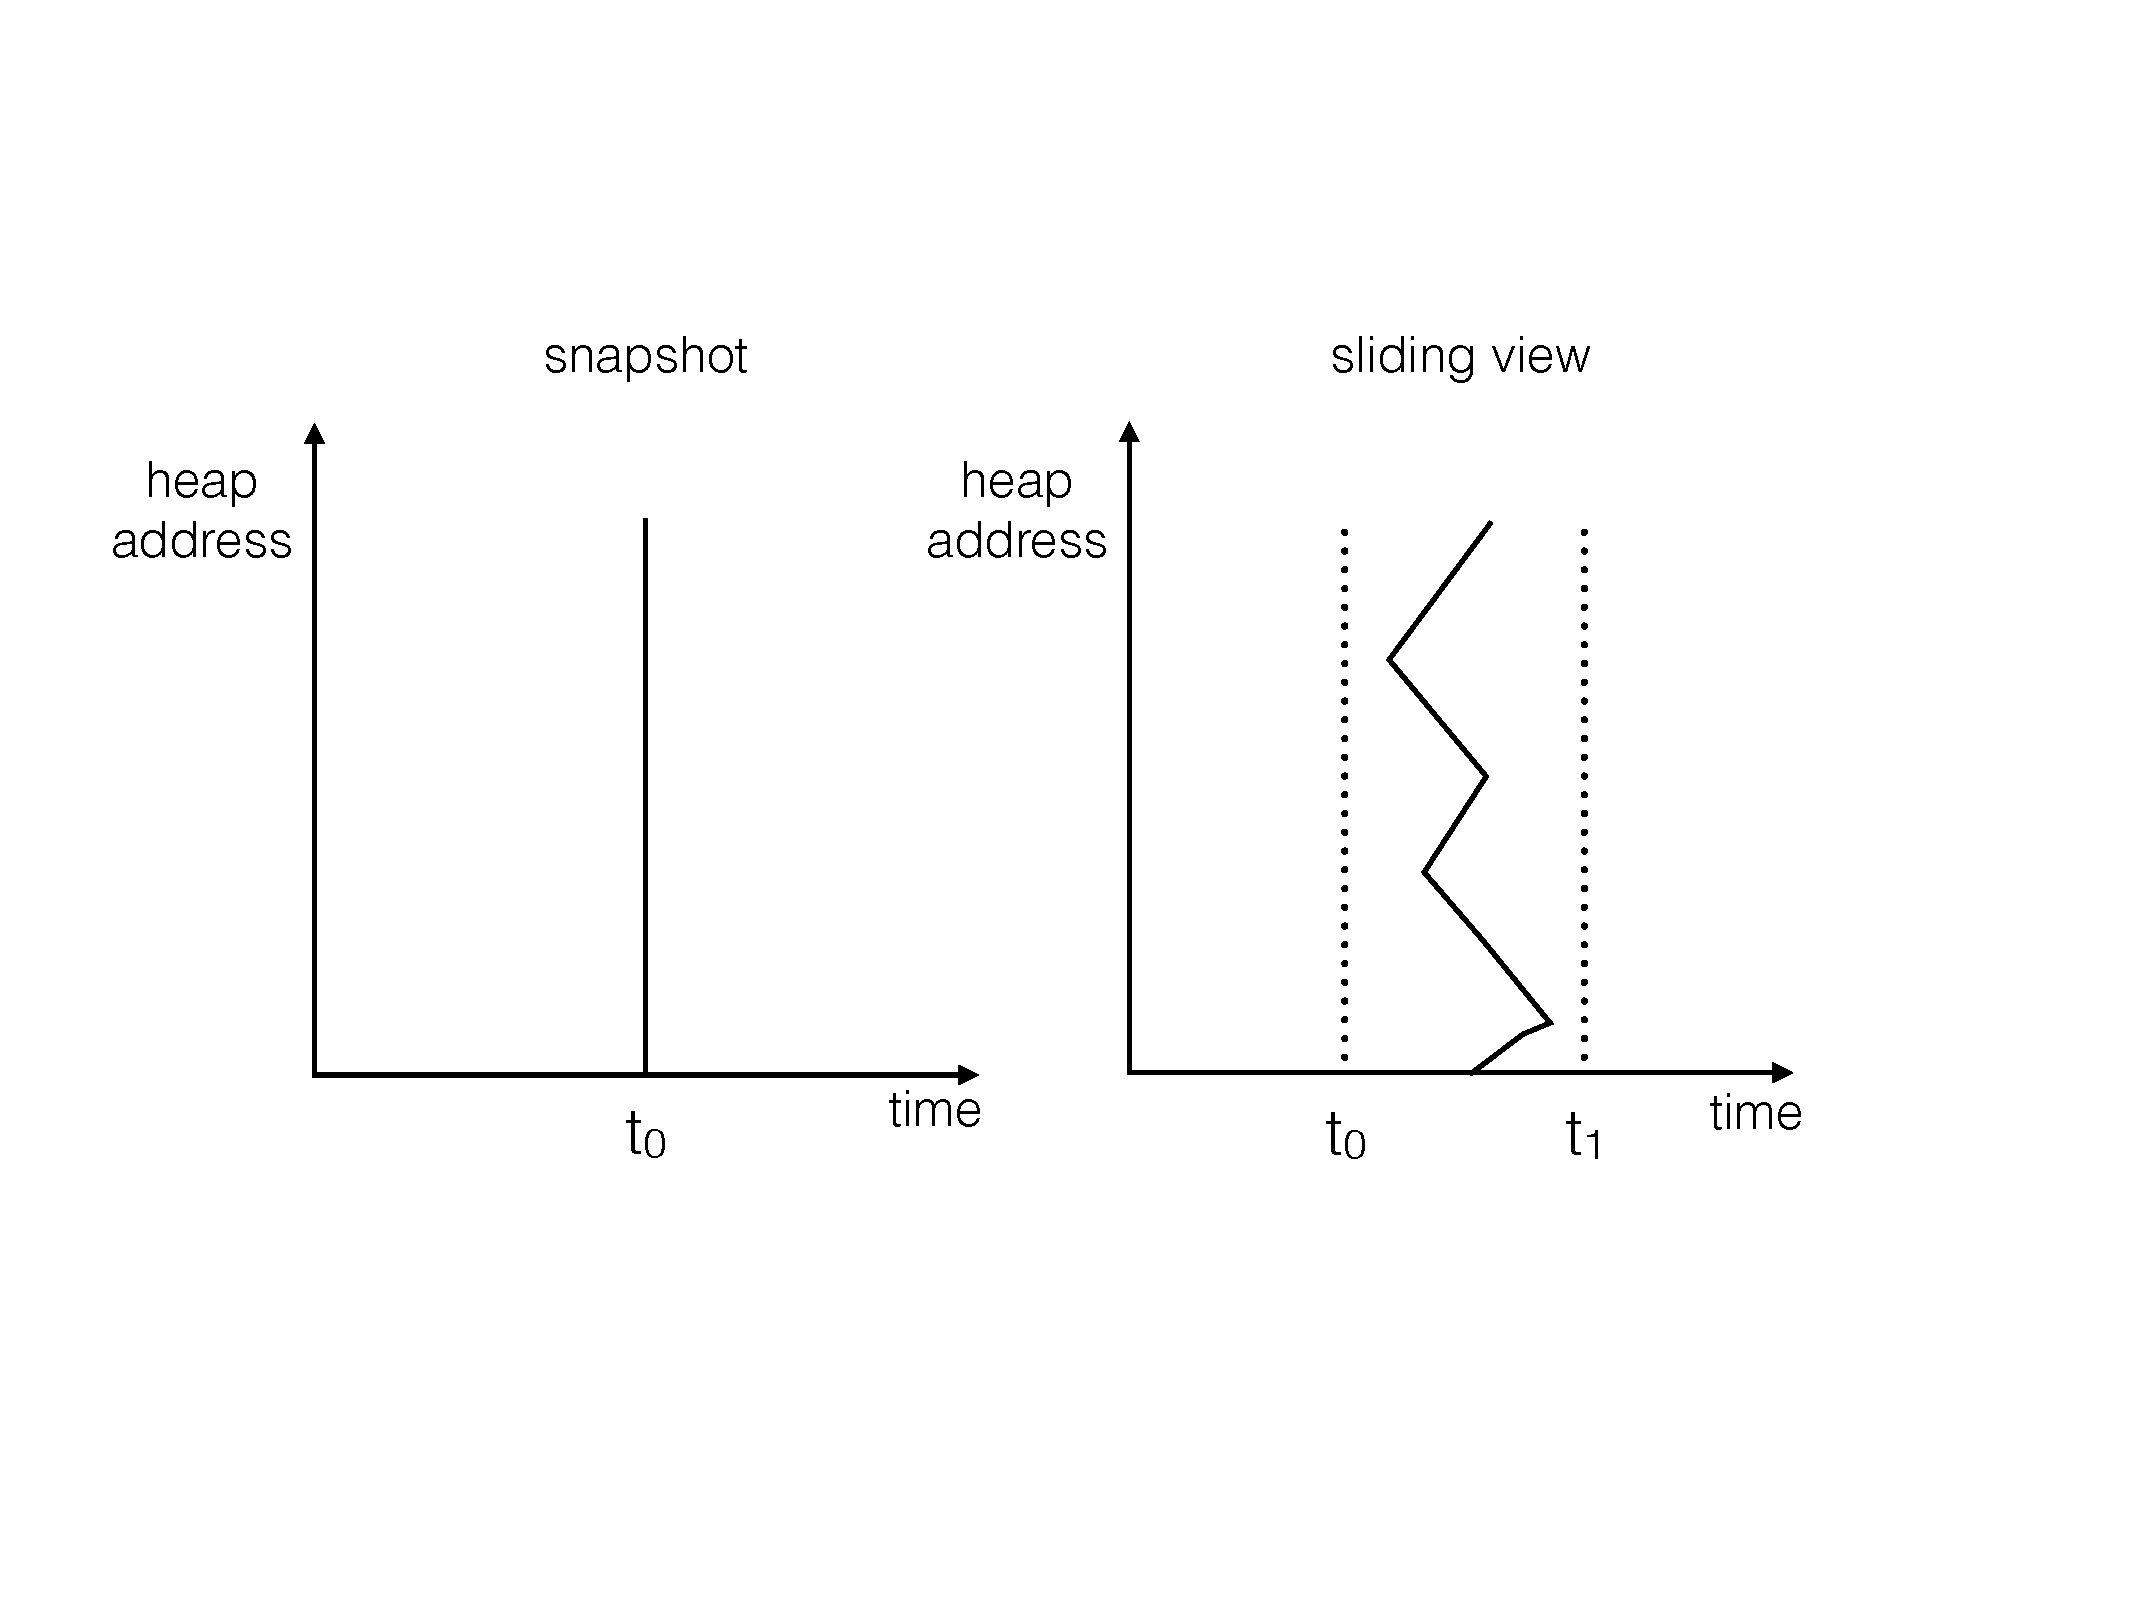
\includegraphics[width=350pt]{snapshot_sliding.pdf}
\end{frame}

\begin{frame}
    \frametitle{On-the-fly sliding views collector}
    Extra precautions needed:
    \begin{itemize}
        \item Can't collect objects to which new reference
              has been created during cycle collection.
        \item To fix this problem a \textit{snooping} mechanism is
              introduced. It effectively pins all such objects.
    \end{itemize}
\end{frame}

\begin{frame}[fragile]
    \frametitle{On-the-fly sliding views collector}
    Modified write barrier with snooping:
    \begin{verbatim}

        Procedure Update(s: Slot, new: Object)
        begin
            local old := read(s)
            if not Dirty(s) then
                Buffer_i[CurrPos_i] := <s, old>
                CurrPos_i := CurrPos_i + 1
                Dirty(s) := true
            write(s, new)
            if Snoop_i then
                Locals_i := Locals_i + new
        end
    \end{verbatim}
\end{frame}

\begin{frame}
    \frametitle{2. Concurrent cycle collection in ref. counted systems}
    \begin{itemize}
        \item
            Introduces two collectors: extremely efficient synchronization-free
            stop-the-world one and less efficient concurrent one.
        \item
            Synchronous collector cleans up the cycles starting from suspected
            cycle roots in $O(N + E)$.
        \item
            Linear performance obtained through single graph traversal
            that colors graph as it goes through it.
        \item
            Sufficient constant benefits by special treatment of acyclic
            data structures.
    \end{itemize}
\end{frame}

\begin{frame}
    \frametitle{3. Age-oriented concurrent garbage collection}
    \begin{itemize}
        \item
            Develops idea of generational collection into on-the-fly setting.
        \item
            Age-oriented is defined as:
            \begin{enumerate}
                \item \textit{Always collects the entire heap}.
                \item During collection treats each generation differently.
            \end{enumerate}
        \item
            Mark-and-sweep for young generation and on-the-fly reference
            counting for the old generation.
    \end{itemize}
\end{frame}

\begin{frame}
    \frametitle{Efficient on-the-fly collection: cr\`eme de la cr\`eme}
    \begin{itemize}
        \item
            Low pause times thanks to sliding views.
        \item
            Efficient cycle collection through a single traversal.
        \item
            Generational with dynamically sized young generation
            that is handled by mark-and-sweep tracing collector.
    \end{itemize}
\end{frame}

\begin{frame}
    \frametitle{State of memory management}
    \definecolor{alizarin}{rgb}{0.82, 0.1, 0.26}
    \definecolor{seagreen}{rgb}{0.18, 0.55, 0.34}
    \newcommand{\Best}{{\color{seagreen} Good}}
    \newcommand{\Worst}{{\color{alizarin} Bad}}
    \begin{center}
        \begin{tabular}{c | c | c | c | c}
                                   & Manual & Regions & Ownership & GC     \\
                                   \hline
            Performance            & \Best  & \Best   & \Best     & \Worst \\
            Predictability         & \Best  & \Best   & \Best     & \Worst \\
            Notational convenience & \Best  & \Worst  & \Worst    & \Best  \\
            Safety                 & \Worst & \Best   & \Best     & \Best

        \end{tabular}
    \end{center}
\end{frame}

\begin{frame}
    \begin{center}
        {\LARGE Research proposal}
    \end{center}
\end{frame}

\begin{frame}
    \frametitle{Research proposal}
    Develop memory management system where:
    \begin{itemize}
        \item
            Application developers don't need to worry about memory
            management.
        \item
            Expert library developers are able to tune their projects
            by providing fine-grain memory management hints that
            exploit domain knowledge for their projects.
    \end{itemize}
\end{frame}


\begin{frame}
    \frametitle{Research proposal}
    \begin{itemize}
        \item
            Low-pause on-the-fly GC as a baseline
        \item
            Optional region annotations to hint at
            expected object lifetimes for performance
            critical sections of code.
        \item
            Effectively "programmable" garbage collection.
    \end{itemize}
\end{frame}
